\chapter{Algorithmen zur Erkennung von SLTRs}

Im vorherigen Kapitel wurden Kriterien für die Existenz einer SLTR erarbeitet, die allerdings nicht sofort einen Algorithmus, sowohl zur Frage nach der Existenz, als auch zum Erlangen einer spezifischen SLTR liefern. Diesem Thema wollen wir uns nun in diesem Kapitel zuwenden und dafür zum Einstieg einen von Aerts und Felsner in \cite{af15} erarbeiteten Algorithmus betrachten.

\section{SLTRs via Zwei-Fluss}

Wir betrachten im folgenden gerichtete Graphen. Das Ziel ist es, für einen gegebenen Graphen sowohl einen Schnyder Wood als auch ein FAA jeweils als Lösung eines Fluss-Problems zu erhalten und diese beiden dann in einem Zwei-Fluss-Problem zu kombinieren, sodass eine Lösung ein Ecken-Kompatibles-Paar gibt und wir somit eine SLTR erhalten. Wir beschäftigen uns also mit der folgenden Problemstellung.

\begin{definition}[Gerichtetes-Multi-Fluss-Problem]
Sei $D=(V,E)$ ein gerichteter Graph, im Weiteren auch Netzwerk genannt, mit den Kapaziäten $c:E\mapsto\mathbb{R}_{+}$, Paaren von ausgezeichneten Knoten $\{(s_1,t_1), ... ,(s_n,t_n)\}$ und positiven Bedarfen $\{d_1, ... ,d_n\}$, dann ist $\varphi=(\varphi_1, ... ,\varphi_n)$ ein zulässiger Fluss, falls
\begin{itemize}
\item[F1] $\forall (u,v) \in E : \sum_{i=1}^{n}{\varphi_i(u,v)} \leq c(u,v) $
\item[F2] $ \forall u \neq s_i,t_i : \sum_{w \in V} \varphi_i(u,w) - \sum_{w \in V} \varphi_i(w,u) $
\item[F3] $ \forall s_i : \sum_{w \in V} \varphi_i(s_i,w) - \sum_{w \in V} \varphi_i(w,s_i) = d_i $
\item[F4] $ \forall t_i : \sum_{w \in V} \varphi_i(w,s_i) - \sum_{w \in V} \varphi_i(s_i,w) = d_i $
\end{itemize}
\end{definition}

\begin{remark}
Im Fall $n=1$ und Kapazitäten $c:E\mapsto\mathbb{N}$ impliziert die Existenz eines zulässigen Flusses die Existenz einer ganzzahligen Lösung, sowohl für gerichtete als auch ungerichtete Graphen, und diese lässt sich in polynomineller Zeit bestimmen. Für $n=2$ und ungerichtete Graphen gilt dies nach \cite{hu} ebenfalls. Für uns im Folgenden interessant wäre jedoch, wie wir sehen werden, der Fall $n=2$ für gerichtete Graphen. Leider ist hier im Allgemeinen die Lösung nur über Lineare Programmierung möglich und befindet sich somit in $\mathcal{NP}$.
\end{remark}

\subsection{Schnyder-Wood-Fluss}

Um einen Schnyder Wood als Fluss-Problem zu kodieren, kann man die in Abschnitt \ref{alpha_orientations} eingeführten $\alpha_s$-Orientierungen auf dem Abschluss von $G+G^*$ nutzen. Fusy zeigt in \cite{fusy07} im Zuge der Untersuchung spezifischer $\alpha$-Funktionen, dass sich $\alpha_s$-Orientierungen von $G+G^*$ in linearer Zeit berechnen lassen, sodass wir auch einen Schnyder Wood auf $G$ in linearer Zeit erhalten.\\

Machen wir uns also an die Konstruktion eines Netzwerks $\mathcal{N}_S$ mit einer Quelle und Senke, sodass eine zulässige Lösung $\varphi_S$ einer $\alpha_s-Orientierung$ von $\tilde{G}$ entspricht, und somit auch einen Schnyder Wald auf $G$ liefert. Besonderes Augenmerk ist hier auf die Möglichkeit einer späteren Kombination mit einem FAA Fluss gelegt, um ein Kombiniertes Netzwerk zu erstellen, und nicht unbedingt auf Effizienz.\

Wie oben schon erwähnt ist $\tilde{G}$ bipartit, Kanten-Knoten haben Grad 4, Knoten-Knoten Grad $deg(v)$ und Gebiets-Knoten Grad $|f|$. Für eine $\alpha_s$-Orientierung muss jeder Kanten-Knoten Ausgrad 1, jeder Knoten-Knoten Eingrad $deg(v)-3$ und jeder Gebiets-Knoten Eingrad $|f|-3$ haben. Die Kanten-Knoten am äusseren Gebiet sind in $\tilde{G}$ immer nach aussen orientiert. Somit müssen wir nur die inneren Kanten-Kanten $E_{in}$ betrachten. \

\begin{figure}[h]
	\centering
  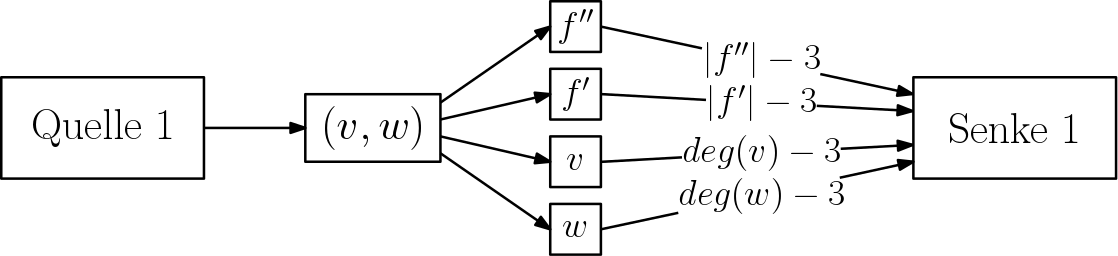
\includegraphics[width=0.9\textwidth]{schnyder_flow.png}
  \caption{Der Schnyder Wood Fluss durch eine innere Kante $(v,w)$.}
  \label{schnyder_flow}
\end{figure}

Sei $\mathcal{N}_S$ ein Netzwerk mit jeweils einer Quelle $s$ und Senke $t$, Kanten von der Quelle zu jedem $e \in E_{in}$ mit Kapazität 1, Kanten von den Kanten-Knoten $e$ zu inzidenten Knoten-Knoten $v$ und (inneren) Gebiets-Knoten $f \in F_{in}$ in $G$ ebenfalls mit Kapazität 1, Kanten von $f \in F_{in}$ zur Senke mit Kapazitäten $|f|-3$, Kanten von den (inneren) Knoten-Knoten $v \in V_{in} = V \setminus \{a_1,a_2,a_3\}$ zur Senke mit Kapazitäten $deg(v)-3$ und Kanten von den Aufhängungen $a_i$ zur Senke mit Kapazitäten $deg(a_i)-2$. Die letzte Kapazität resultiert aus dem Fakt, dass die Halbkante in $G+G^*$ von $a_i$ aus immer nach aussen orientiert ist und wir somit nur noch zwei andere Kanten nach aussen orientieren müssen.

Der Bedarf des Netzwerkes entspricht der Anzahl der inneren Kanten von $G$. Sei nun $\varphi_S$ eine zulässige ganzzahlige Lösung, dann hat jeder Kanten-Knoten $e$ Ausgrad 1. Der Fluss $\varphi_S$ entlang einer Auskante von $e \in E_{in}$ in $\mathcal{N}_S$ entspricht dann genau der hin zu $e$ orientierten Kante einer $\alpha_{s}$-Orientierung auf $G+G^*$. Die Knoten-Knoten und Gebiets-Knoten haben $deg(v)-3$ bzw. $|f|-3$ von $\varphi_S$ genutzte Auskanten und somit entspricht hier eine leere Kante in $\mathcal{N}_S$ einer von $v$ bzw. $f$ weg orientierten Kante bezüglich $\alpha_{s}$. Ein zulässiger ganzzahliger Fluss $\varphi_S$ kodiert also eine $\alpha_s$-Orientierung auf $G+G^*$. Somit existiert genau dann ein Schnyder Wald auf $G$, wenn eine ganzzahlige Lösung $\varphi_S$ für $\mathcal{N}_S$ existiert.

\subsection{FAA-Fluss}\label{faa-flow}

Um ein FAA für einen planaren Graphen $G$ zu erhalten, müssen wir jedem Gebiet $f \in F$ genau drei Ecken und $|f|-3$ flache Winkel zuordnen und jeder Knoten darf maximal einem Gebiet zugeordnet werden, also in diesem flach sein. Falls eine Einbettung und die Aufhängungen $\{a_1,a_2,a_3\}$ gegeben sind, müssen wir jedem inneren Gebiet $f \in F_{in}$ drei Ecken und $|f|-3$ flache Winkel zuweisen und jeder innere Knoten $v \in V_{in}$ darf maximal einem Gebiet zugeordnet werden. Wir konstruieren ein Netzwerk für den zweiten Fall, das sich leicht verallgemeinern lässt.\

Sei also wieder $\mathcal{N}_F$ ein Netzwerk mit einer Quelle und Senke, einem Knoten für jeden inneren Winkel $(f,v)$, mit $v\in V$ und $f \in F_{in}$, Knoten für alle inneren Gebiete $f$ und alle inneren Knoten $v$. Von der Quelle existiert eine Kante mit Kapazität 1 zu jedem inneren Winkel $(f,v)$, von jedem inneren Winkel $(f,v)$ jeweils eine Kante zu $f$ und zu $v$ mit Kapazität 1, von jedem inneren Gebiet $f$ eine Kante mit Kapazität 3 zur Senke und zuletzt noch eine Kante von jedem inneren Knoten $v$ zur Senke mit Kapazität 1. Der Bedarf des Netzwerks ist $\sum_{f \in F_{in}}{|f|}$ und entspricht der Anzahl der inneren Winkel von $G$. 

\begin{figure}[h]
	\centering
  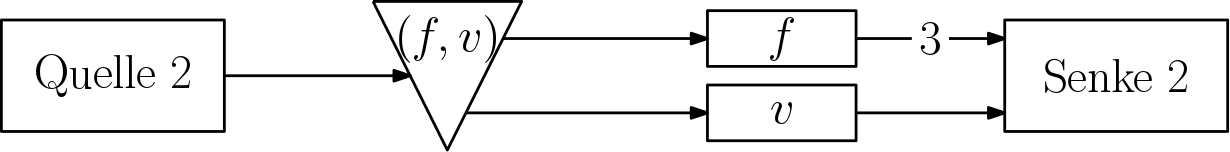
\includegraphics[width=0.8\textwidth]{faa_flow.png}
  \caption{Der FAA-Fluss durch einen Winkel $(f,v)$.}
  \label{faa_flow}
\end{figure}


Sei $\varphi_F$ ein zulässiger ganzzahliger Fluss, dann entspricht Fluss auf einer Kante $((f,v),f)$ einer Ecke (eines möglichen GFAAs) von $f$ und Fluss auf $((f,v),u)$ der Zuweisung eines Knoten zu $f$, also einem flachen Winkel in einem GFAA. Zur Vereinfachung sprechen wir im Weitern auch von Ecken- respektive Zuweisungs-Fluss. Somit wird jeder innere Winkel entweder dem Gebiet zugewiesen oder als Ecke ausgezeichnet und es kann nur jeweils ein Winkel an jedem inneren Knoten zugewiesen werden. $\varphi_F$ respektiert also die Bedingungen aus Definition \ref{def_faa} und es existieren nur dann FAAs auf $G$, wenn mindestens eine ganzzahlige Lösung für $\mathcal{N}_F$ existiert. Eine spezifische Lösung $\varphi_F$ entspricht genau einem FAA auf $G$.

\begin{remark}

Das oben konstruierte Netzwerk zur Bestimmung von FAAs lässt sich auch als Zwei-Fluss Problem konstruieren, wenn wir für Ecken- und Zuweisungs-Fluss getrennte Quellen und Senken einführen. Der Bedarf des Ecken-Flusses ist dann $3|F_{in}|$ und der Bedarf des Zuweisung-Flusses $\sum_{f \in F_{in}}{|f|-3}$.

\begin{figure}[h]
	\centering
  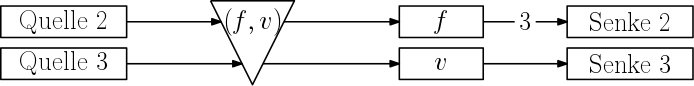
\includegraphics[width=0.8\textwidth]{faa_2_flow.png}
\end{figure}

Eine zulässige ganzzahlige Lösung $\varphi_F = (\varphi_{F_2},\varphi_{F_3})$ entspricht dann wieder einem FAA auf $G$, da aus der Ganzzahligkeit folgt, dass ein Winkel entweder von $\varphi_{F_2}$ oder $\varphi_{F_3}$ genutzt wird und somit eine Definition \ref{def_faa} respektierende Beschriftung der Winkel vorliegt.

\end{remark}




\subsection{Graphen mit wenigen FAAs oder Schnyder Woods}

Wir wollen in diesem Abschnitt kurz betrachten, wie wir 
Sei $G$ ein intern-3-zusammenhängender Graph 
Für Graphen mit wenigen FAAs oder wenigen Schnyder Woods\footnote{Es sind hier maximal polynominell viele gemeint.} liefern die Ansätze oben jeweils Wege in polynomineller Zeit zu verifizieren, ob SLTRs existieren und ein Gutes-FAA zu erhalten. Die Graphen mit nur genau einen Schnyder Wood wurden von Felsner und ... TODO 

\subsection{Ein Zwei-Fluss Netzwerk zur Erkennung von SLTRs}

Im Verlauf des Kapitels haben wir nun sowohl für Schnyder Woods als auch für FAAs ein Netzwerk betrachtet, für das eine ganzzahlige Lösung einen Schnyder Wood bzw. ein FAA für einen planen Graphen $G$ liefert. Wir wollen jetzt eine Kombination aus beiden erstellen die ein Ecken kompatibles Paar $(\sigma,\phi)$ aus einem Schnyder Labeling $\sigma$ und einem FAA $\phi$  kodiert.\

Es folgt die Konstruktion eines Netzwerkes, wir bezeichnen es mit $\mathcal{N}_G$, welches diesen Wunsch erfüllt, für das eine ganzzahlige Lösung ein Ecken kompatibles Paar kodiert und somit nach Theorem \ref{theo_coco} eine SLTR für $G$ existiert. Leider handelt es sich hierbei um ein 2-Fluss-Netzwerk, aber darauf wollen wir später genauer eingehen.\\

Wie oben in Abschnitt \ref{faa-flow} erwähnt lässt sich ein FAA auch mit einem Zwei-Fluss kodieren und wir können Ecken- und Zuweisungs-Fluss mit den passenden Bedarfen getrennt betrachten. Wir müssen jetzt diese drei Flüsse, also Schnyder-, Ecken- und Zuweisungs-Fluss in einem Netzwerk kombinieren. In \cite{af15} ergeben Schnyder- und Ecken-Fluss zusammen Fluss von Typ 1 und der Zuweisungs-Fluss Typ 2. Wir wollen hier analog ein Netzwerk konstruieren in dem wir FAA und Schnyder-Wood Fluss nicht trennen. Der Verständlichkeit halber werden wir Pfade, die in einer Lösung von einem der drei Flussarten genutzt werden, \textit{Schnyder-Pfad, Ecken-Pfad} und \textit{Zuweisungs-Pfad} nennen.\\

Bei der Kombination der beiden oben konstruierten Netzwerke $\mathcal{N}_S$ und $\mathcal{N}_F$ zu $\mathcal{N}_G$ müssen wir die Ecken Kompatibilität gewährleisten. K1 zu erfüllen, also die Nutzung der gleichen Aufhängungen von $\sigma$ und $\phi$, ist kein Problem. Allerdings müssen wir für K2 das Netzwerk etwas komplizierter machen. Betrachten wir als Basis $\mathcal{N}_S \cup \mathcal{N}_F$ und fürs erste nur ein inneres Gebiet $f$, dann sehen wir, dass es $|f|-3$ Schnyder-Fluss aufnimmt, aber $|f|$ Einkanten in $\mathcal{N}_S$ hat, es sind also genau die drei nötigen Kanten für den Ecken-Fluss aus $\mathcal{N}_F$ übrig. Wir müssen gewährleisten, dass jede Ecke im Schnyder Labeling ein anderes Label hat. Betrachten wir also den von $\varphi_S$ induzierten Schnyder Wood auf $G^*$. Nach \cite{felsner12} können wir diesen aus der $\alpha_S$-Orientierung ablesen. 

\begin{figure}[h]
	\centering
  	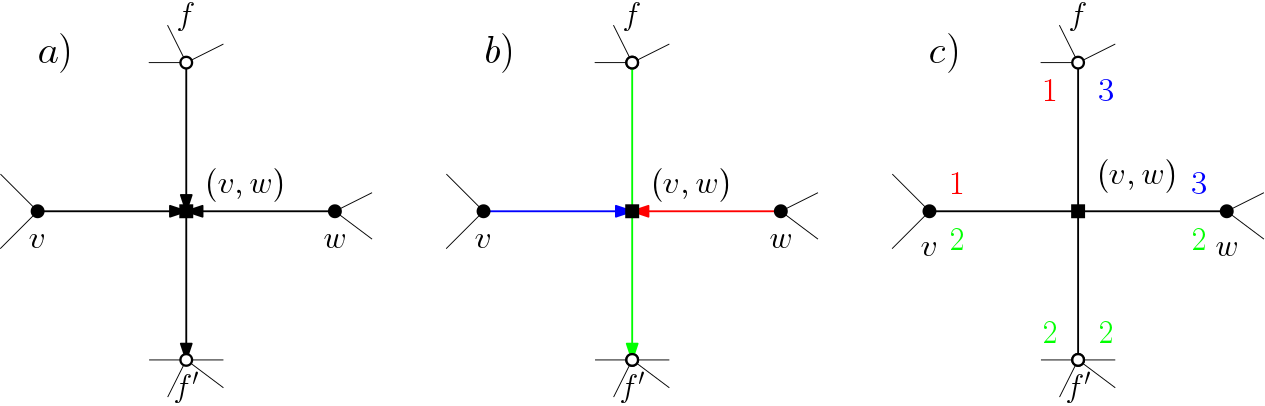
\includegraphics[width=0.7\textwidth]{alpha_bij.png}
  	\caption{a) Eine $\alpha_s$-Orientierung um eine innere Kante von $G$. b) Teile der korrespondierenden Schnyder Woods auf $G$ und $G^*$. c) Die induzierten Label, die für $G$ und $G^*$ gleich sind.}
	\label{alpha_bij}
\end{figure}

Es gilt außerdem, wie in Abbildung \ref{alpha_bij} skizziert, dass die Label der Ecke eines Gebietes in $G$ und das ihr in $G+G^*$ gegenüberliegenden Label der Ecke eines Gebiets um einen Knoten in $G^*$ gleich sind. Für eine zu $v$ in $G^*$ hin orientierte Kante folgt aus der Bijektion zwischen Schnyder Labelings und Schnyder Woods aus Abschnitt \ref{sw}, dass die Label links und rechts am Ende dieser Kante gleich sind. Somit sind auch die Label in $G$ gleich und wir können die folgende Eigenschaft festhalten.
\begin{itemize}
\item [A1] Die Label, des von $\alpha_s$ induzierten Schnyder Wood auf $G$, sind zwischen zwei aufeinander folgenden zu $f$ orientierten Kanten gleich.
\end{itemize}
Da es genau drei zu $f$ orientierte Kanten gibt müssen wir also dafür sorgen, dass für jedes Paar dieser Kanten eine Ecke zwischen ihnen liegt, da so die drei Ecken unterschiedliche Label haben und wir K2 erfüllen. Um dies zu erlangen implementieren wir eine zyklische Struktur um jedes innere Gebiet, wie in Abbildung \ref{comb_face_sketch} skizziert.\\

\begin{figure}[h]
	\centering
  	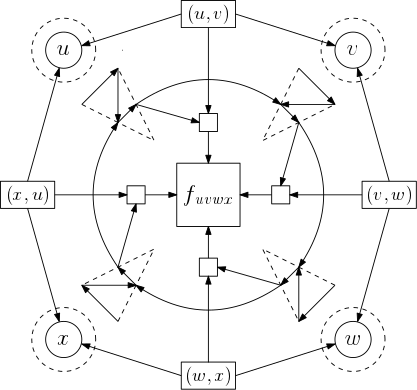
\includegraphics[width=0.9\textwidth]{combined_face_sketch.png}
  	\caption{Eine Skizze des kombinierten Netzwerkes auf einem inneren Gebiet mit $|f| = 4$. Beispielhaft sind Schnyder-Fluss (rot), Ecken-Fluss (blau) und Zuweisungs-Fluss (grün) eingezeichnet. }
	\label{combined_face_sketch}
\end{figure}

Betrachten wir zuerst den Schnyder-Fluss. Dieser wird Fluss von Typ 1, also von Quelle 1 zu Senke 1 sein. Für einen Schnyder-Pfad der durch einen Knoten $v$ führt hat sich nichts geändert. Der in der Skizze eingezeichnete Schnyder-Pfad der durch $f$ führt passiert davor einen extra Knoten, wir nennen ihn \textit{kleines Quadrat} der gewährleisten soll, dass von Seite des Gebietes aus entweder ein Schnyder-Pfad oder ein Ecken-Pfad in $f$ mündet. Zuletzt fügen wir wie oben von jedem inneren Gebiet eine Kante mit Kapazität $|f|-3$ zu Senke 1 ein. Somit kodiert hier eine ganzzahlige Lösung weiterhin einen Schnyder Wood auf $G$.\

Kommen wir nun zum FAA-Fluss, also Fluss von Typ 2. Von Quelle 2 geht genau wie in Abbildung \ref{faa_flow} eine Kante zu jedem inneren Winkel $(f,v)$. Ein Zuweisungs-Pfad verlässt diesen Winkel über einen zusätzlich zu $v$ eingefügten Dummy-Knoten $v^*$. Von jedem $v^*$ geht eine Kante mit Kapazität 1 zu einer Dummy-Senke und von dieser eine Kante mit Kapazität $\sum_{f \in F_{in}} |f|-3$ zu Senke 2, wie in Abbildung \ref{dummy_sink} illustriert.

Die Dummy-Knoten sorgen dafür, dass jeder Knoten im FAA nur einmal zugewiesen werden kann, ohne in Konflikt mit dem Schnyder-Fluss zu kommen, und die eingeschobene Dummy-Senke beschränkt die Anzahl der zugewiesenen Knoten, genau wie im zuvor konstruierten FAA-Fluss, auf $\sum_{f \in F_{in}} |f|-3$.
\begin{figure}[h]
	\centering
  	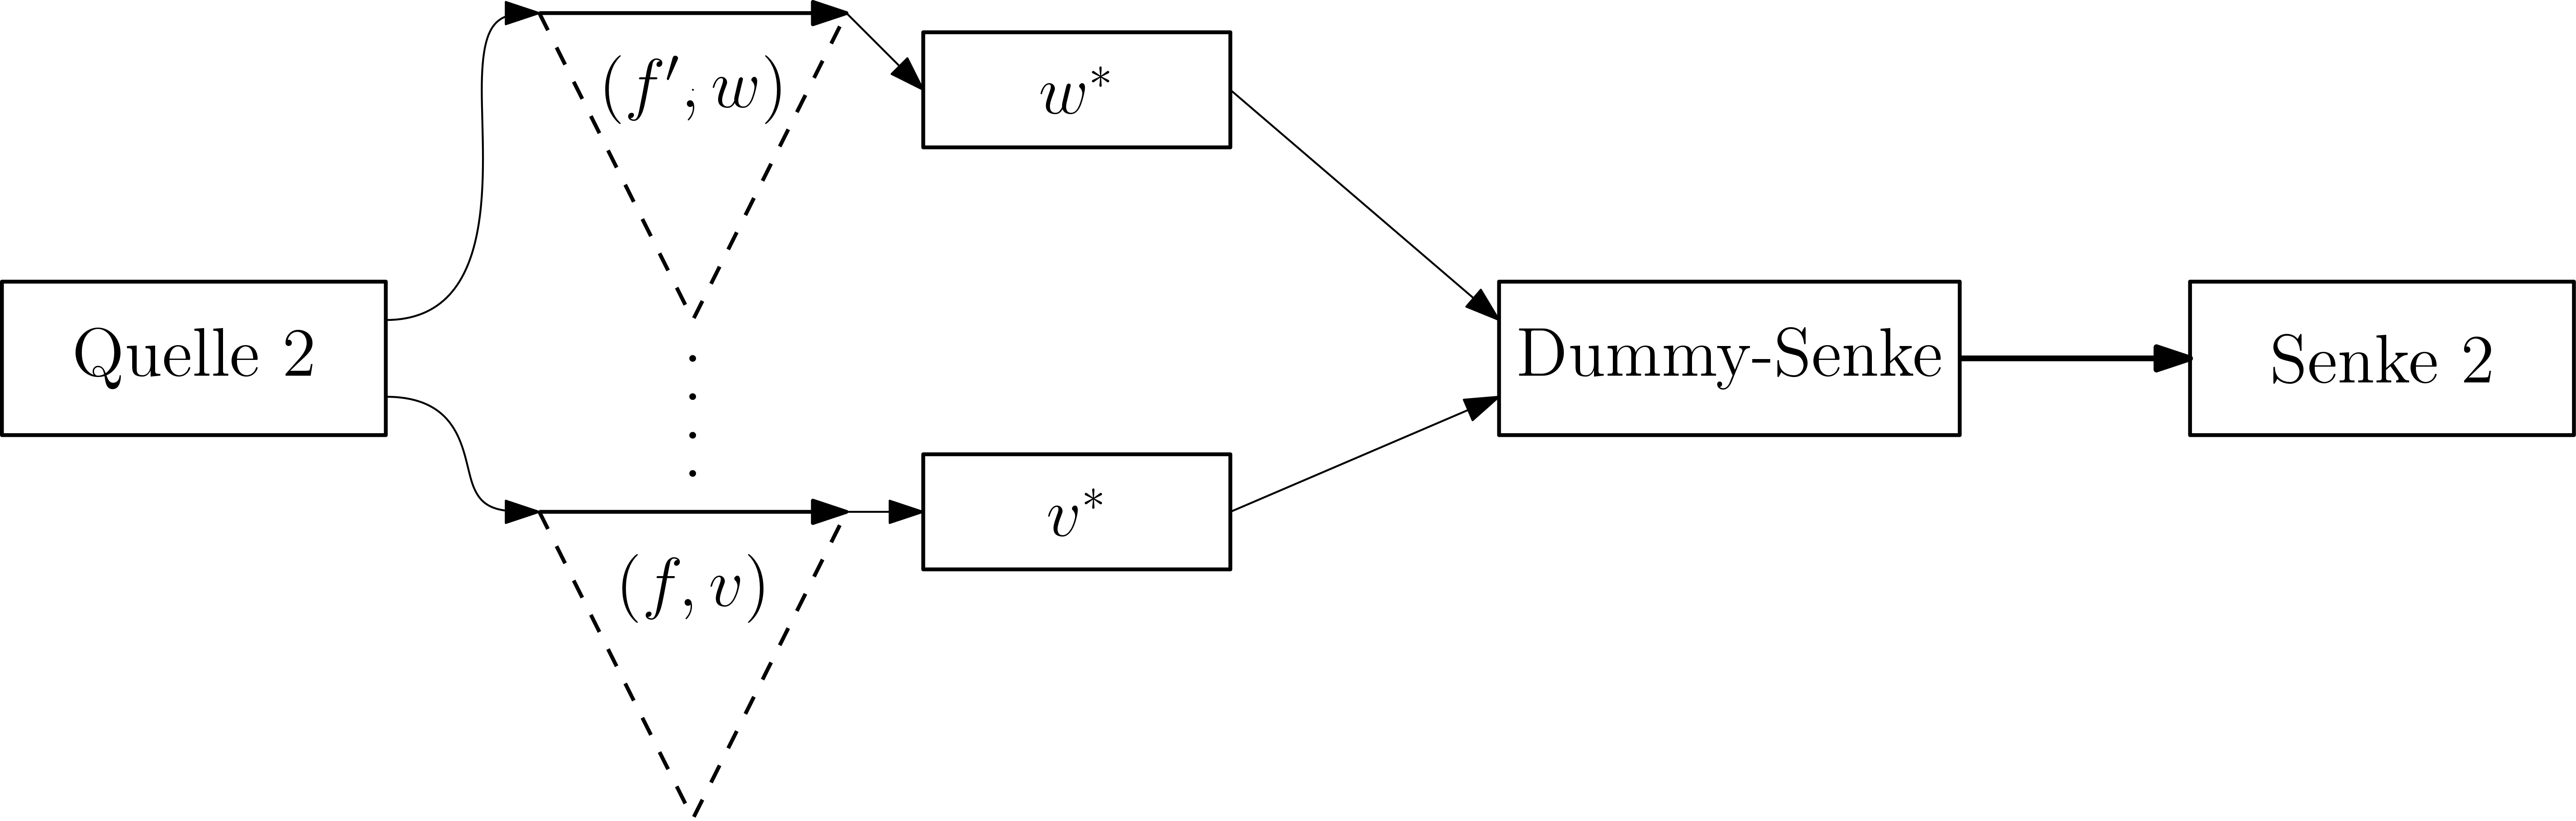
\includegraphics[width=0.7\textwidth]{dummy_sink.png}
  	\caption{Der Zuweisungsfluss durch die Winkel, Dummy-Knoten und die zusätzliche Kante vor Senke 2. Die Kante rechts hat Kapazität $\sum_{f \in F_{in}} |f|-3$ und alle anderen Kapazität 1.}
	\label{dummy_sink}
\end{figure}
Es bleibt der Ecken-Fluss. Hier betritt der Pfad wieder durch einen Winkel das Gebiet $f$ und muss es über ein ungenutztes kleines Quadrat verlassen. Die zweite und dritte Kante in jedem Winkeldreieck gewährleisten, dass nicht immer das nächste kleine Quadrat genutzt werden muss. Falls dies von Schnyder-Fluss besetzt ist und der nächste Winkel zugewiesen wird, dann kann ein Ecken-Pfad den nächsten Winkel passieren. Weiter sorgt die erste Kante, die von sowohl Schnyder-, als auch Winkel-Pfaden genutzt werden kann für eine eindeutige Beschriftung (als Ecke oder nicht) im Falle einer ganzzahligen Lösung. Wie oben existieren auch hier Kanten von jedem inneren Gebiet zu Senke 2 mit Kapazität drei.\\

Betrachten wir die Bedarfe der beiden Flüsse von Typ 1 und Typ 2, $\varphi_1$ bzw. $\varphi_2$. Beide entsprechen jeweils den Bedarfen der oben konstruierten $\mathcal{N}_S$ und $\mathcal{N}_F$, da nur so, mit den gleichen Argumenten wie zuvor, ein Schnyder Wood und ein FAA kodiert werden können. Jedes Gebiet benötigt genau drei Ecken und $|f|-3$ zugewiesene Knoten und der je ein Schnyder-Pfad führt durch jede innere Kante, $|E_{in}|$. Hier seien wieder $E_{in}$ die inneren Kanten und $F_{in}$ die inneren Gebiete von $G$. Es gilt also:

\begin{itemize}
\item $d_1$ = Bedarf$(\varphi_1) = $ Bedarf$(\varphi_S) = |E_{in}|$
\item $d_2$ = Bedarf$(\varphi_2) = $ Bedarf$(\varphi_F) =  \sum_{f \in F_{in}}(|f|-3) + 3|F_{in}| = \sum_{f \in F_{in}} |f|$
\end{itemize}

Bevor wir in Theorem \ref{theo_algo} zeigen, dass eine ganzzahlige Lösung $\varphi=(\varphi_1,\varphi_2)$ auch wirklich ein Ecken kompatibles Paar kodiert wollen wir noch ein Paar weitere Beobachtungen festhalten. Nehmen wir also an wir haben eine ganzzahlige Lösung $\varphi$ gefunden, dann gilt für diese:
\begin{itemize}
\item [A2] Jede äussere Kante in einem Winkel-Dreieck ist ausgelastet, sie wird entweder von einem Ecken- oder Zuweisungspfad genutzt.
\item [A3] Jede Kante von einem kleinen Quadrat zu einem inneren Gebiet $f$ ist ausgelastet, sie wird entweder von einem Schnyder- oder Ecken-Pfad genutzt.
\item [A4] Ein inneres Gebiet $f$ mit $|f|=3$ kann nicht von Zuweisungs- bzw. Schnyder-Pfaden genutzt werden.
\end{itemize}

Wir wollen diese Beobachtungen kurz begründen. Für jede mögliche ganzzahlige Lösung $\varphi$ gilt $$|\varphi|=|\varphi_1|+|\varphi_2| = |E_{in}| + \sum_{f \in F_{in}} |f|.$$
Da es genau $\sum_{f \in F_{in}} |f|$ innere Winkel gibt und der FAA-Fluss $\mathcal{N}_G$ nur durch diese betreten kann ergibt sich A2. A3 wird aus Gleichung \ref{eq_sat} weiter unten folgen. Durch ein inneres Gebiet $f$ müssen drei Ecken-Pfade führen und im Fall $|f|=3$ führt dies zu A4, da kein Platz in den Winkeln für Zuweisungs-Pfade und keine freien kleinen Quadrate für Schnyder-Pfade existieren.

\begin{theorem}\label{theo_algo}
Sei $G$ ein intern-3-zusammenhängender Graph mit gegebenen Aufhängungen $\{a_1,a_2,a_3\}$, dann existiert eine SLTR von $G$, genau dann wenn ein ganzzahliger zulässiger Fluss $\varphi=(\varphi_1,\varphi_2)$ auf $\mathcal{N}_G$ existiert.
\end{theorem}

\begin{proof}
Sei $G$ ein intern-3-zusammenhängender Graph mit Aufhängungen $\{a_1,a_2,a_3\}$ und $\varphi=(\varphi_1,\varphi_2)$ sei ein ganzzahliger machbarer Fluss auf $\mathcal{N}_G$. In einem ersten Schritt extrahieren wir einen Schnyder-Wood $\sigma$ und ein FAA $\phi$ um dann zu zeigen, dass sie ein Ecken kompatibles Paar bilden. Für einen machbaren Fluss müssen die Bedarfe erfüllt werden. Es gilt somit $|\varphi_1| =  |E_{in}|$ und $|\varphi_2| = \sum_{f \in F_{in}} |f|$.
\begin{equation}\label{eq_sat}
\begin{split}
|\varphi_1| + |\varphi_2| & = \sum_{f \in F_{in}} (|f|-3) + 3|F_{in}| + |E_{in}|\\
		& = \sum_{f \in F_{in}} (|f|-3) + 2|E| -|V| - 1 + 2|F| - |f_{aus}|\\
		& = \sum_{f \in F_{in}} (|f|-3) + \sum_{v \in V} (deg(v)-3) + 2|V| + 2|F| - 1 - |f_{aus}|\\
		& = \sum_{f \in F_{in}} (|f|-3) + \sum_{v \in V} (deg(v)-3) + 2|E| + 3 - |f_{aus}|\\
		& = \underbrace{\sum_{f \in F_{in}}(|f|-3)  }_{\text{\parbox{8em}{Dummy-Senke zu Senke 2}}} + \underbrace{\sum_{v \in V} (deg(v)-3) +3 }_{\text{\parbox{10em}{Kapazität Senke 2 von den Knoten.}}} +\underbrace{\sum_{f \in F_{in}}(|f|-3) + 3|F_{in}|}_{\text{\parbox{12em}{Kanten von den Quadraten zu den inneren Gebieten}}}
\end{split}
\end{equation}

Die beiden Terme in der rechten unteren Klammer entsprechen den Kapazitäten von den inneren Gebieten zu Senke 1 und Senke 2. Somit sind alle Kanten zu den Senken ausgelastet und die Kanten von den kleinen Quadraten zu den inneren Gebieten sind ebenfalls ausgelastet. Diese sind die einzigen Kanten in $\mathcal{N}_G$ die sowohl von $\varphi_1$ als auch $\varphi_2$ genutzt werden können. Kapazität eins und Ganzzahligkeit von $\varphi$ impliziert somit A3.\\

Beginnen wir mit $\varphi_1$ um einen Schnyder Wood, oder genauer eine $\alpha_s$-Orientierung, zu erhalten. $|\varphi_1| = |E_{in}|$, somit führt durch jede innere Kante ein Schnyder-Pfad und dieser gibt uns die nach aussen gerichtete Kante in $\alpha_s$. Es bleibt zu zeigen, dass für jedes innere Gebiet und jeden Knoten die Bedingungen aus Theorem \ref{alpha_bij} für eine $\alpha_s$ eingehalten werden. Da alle Kanten von den Knoten zu Senke 1 ausgelastet sind folgt, dass durch jeden inneren Knoten $v$ genau $deg(v)-3$ Schnyder-Pfade führen. Somit ergeben die leeren Einkanten von $v$ in $\mathcal{N}_G$ die drei Auskanten für $\alpha_s$. Für eine Aufhängung $a_i$ folgt analog, dass die beiden ungenutzten Einkanten, zusammen mit der Halbkante ins äußere Gebiet, die Bedingungen der $\alpha_s$-Orientierung erfüllen. Es bleibt zu zeigen, dass durch jedes innere Gebiet $|f|-3$ Schnyder-Pfade führen. Der restliche Schnyder-Fluss $|E_{in}| - \sum_{v \in V} (deg(v)-3)$ muss durch die inneren Gebiete führen und aus der ersten und letzten Zeile von Gleichung \ref{sat_eq} folgt $$|E_{in}| - \sum_{v \in V} (deg(v)-3) = \sum_{f \in F_{in}} (|f|-3).$$
Somit führen $|f|-3$ Schnyder-Pfade durch jedes innere Gebiet und wir können die $\alpha_s$-Orientierung vervollständigen und erhalten einen Schnyder Wood auf $G$.\\

Betrachten wir nun $\varphi_2$. Nach A4 sind alle äusseren Kanten in den Winkeln ausgelastet. Falls diese nun in jedem inneren Gebiet von drei Ecken-Pfaden und $|f|-3$ Zuweisungs-Pfaden genutzt werden können wir ein FAA extrahieren. Da alle Kanten zu Senke 2 ausgelastet sind führen $\sum_{f \in F_{in}} (|f|-3)$ Pfade durch die Dummy-Senke. Somit werden auch $\sum_{f \in F_{in}} (|f|-3)$ Knoten inneren Gebieten zugewiesen. Indem wir die Pfade zurückverfolgen und sehen aus welchem Gebiet der Zuweisungs-Pfad einen Dummy-Knoten betritt, können wir diese Informationen auslesen. Es bleibt zu zeigen, dass jedem Gebiet genau $|f|-3$ Knoten zugewiesen werden, dies gilt, genau dann wenn durch jedes Gebiet drei Ecken-Pfade laufen. Da die Kanten von den inneren Gebieten zu Senke 2 ausgelastet sind muss dies allerdings gelten. Wir können also aus $\varphi_2$ ein FAA für $G$ extrahieren. \\

Nun müssen wir zeigen, dass $\sigma$ und $\phi$ ein Ecken kompatibles Paar ergeben. C1, dass beide die gleichen Aufhängungen nutzen folgt sofort aus der Konstruktion von $\mathcal{N}_G$. Es bleibt C2.\

Betrachten wir ein Teilnetzwerk (wie in Abbildung \ref{combined_face_sketch}) um ein inneres Gebiet $f$. Die drei Ecken-Pfade können keine der $|f|-3$ kleinen Quadrate nutzen die schon von Schnyder-Fluss okkupiert werden. Die drei übrigen kleinen Quadrate nennen wir \textit{verfügbar}. Ausgehend von $f$ folgen wir den Ecken-Pfaden rückwärts zu den verfügbaren kleinen Quadraten. Wenn wir das Quadrat verlassen gelangen wir zur dritten Kante eines Winkeldreiecks (entgegen dem Uhrzeigersinn). Nun verlassen wir das Gebiet entweder über diesen Winkel oder bewegen uns weiter (entgegen dem Uhrzeigersinn) zum nächsten Winkeldreieck. Doch wir werden zeigen, dass dies nur dann geschieht wenn das kleine Quadrat zwischen diesen nicht \textit{verfügbar} ist. Also betritt zwischen zwei \textit{verfügbaren} kleinen Quadraten ein Ecken-Pfad das Gebiet und die Winkel haben nach A1 unterschiedliche Label.

\begin{claim}\label{claim1}
Seien $Q_1,Q_2$ und $Q_3$, im Uhrzeigersinn, die drei verfügbaren kleinen Quadrate um ein inneres Gebiet $f$. Dann existiert ein Ecken-Pfad, welcher das Netzwerk über $Q_i$ verlässt, und dieser betritt es in einem Winkel zwischen, im Uhrzeigersinn, $Q_{i-1}$ und $Q_i$.
\end{claim}

Angenommen dies ist nicht der Fall und nehmen wir ohne Beschränkung der Allgemeinheit an, dass der Ecken-Pfad $p$ das Gebiet durch $Q_3$ verlässt. Dann liegt der Winkel über den $p$ das Gebiet betritt nicht zwischen $Q_2$ und $Q_3$. Angenommen er liegt zwischen $Q_1$ und $Q_2$. Betrachte das letzte Winkeldreck vor $Q_2$. Nach unserer Annahme ist die innere Kante dieses Dreiecks von $p$ ausgelastet. Somit kann kein Ecken-Fluss zu $Q_2$ gelangen und wir erhalten einen Widerspruch zu, da alle kleinen Quadrate entweder von Ecken- oder von Schnyder-Fluss genutzt werden müssen. Mir dem gleichen Argument kann $p$ das Gebiet zwischen $Q_3$ und $Q_1$ betreten. Somit stimmt Behauptung \ref{claim1}.

\begin{claim}
Alle Winkel zwischen zwei aufeinander folgenden verfügbaren kleinen Quadraten, haben die selben Label im Schnyder Labeling $\sigma$.
\end{claim}
Diese Behauptung folgt aus der in Abbildung \ref{alpha_bij} illustrierten Bijektion zwischen der $\alpha_S$ Orientierung und den Schnyder Labelings auf $G$ und $G^*$. Die Winkel links und rechts von einem kleinen Quadrat, dass von einem Schnyder-Pfad genutzt wird, haben das gleiche Label in $\sigma$, da diese den Einkanten in $\alpha_s$ entsprechen. Die Auskanten entsprechen den verfügbaren kleinen Quadraten, und hier ändern sich die Label.\\

Diese beiden Behauptungen zusammen zeigen, dass jede Ecke aus $\phi$ ein anderes Label in $\sigma$ hat. Somit handelt es sich um ein Ecken Kompatibles Paar $(\sigma,\phi)$.\\

Wir haben die Rückrichtung gezeigt. Nehmen wir also an, dass eine SLTR für $G$ existiert. Wir müssen nun einen zulässigen ganzzahligen Fluss $\varphi=(\varphi_1,\varphi_2)$ auf $\mathcal{N}_G$ konstruieren, der die SLTR kodiert. Nach Theorem \ref{theo_coco} existiert ein Ecken kompatibles Paar $(\sigma,\phi)$ aus einem Schnyder Labeling $\sigma$ und einem FAA $\phi$, das zu diesem SLTR passt. Betrachte die zu $\sigma$ gehörige $\alpha_s$-Orientierung.

Wir beginnen mit einem leeren, wie oben konstruierten Netzwerk $\mathcal{N}_G$ und waren nun Schritt für Schritt einen zulässigen Fluss $\varphi$ konstruieren.

Zuerst fügen wir für jeden zugewiesenen Winkel einen Pfad von Quelle 2, über die äussere Kante des Winkeldreiecks, den zugehörigen Dummy-Knoten und die Dummy-Senke hin zu Senke 2 ein. Es kommen somit $\sum_{f \in F_{in}}|f|-3$ Einheiten Fluss hinzu und die Kante von der Dummy-Senke zu Senke 2 wird ausgelastet.

Als nächsten fügen wir den, die $\alpha_s$-Orientierung kodierenden Fluss, hinzu. Zuerst von Quelle 1 zu jeder inneren Kante $e$, dann von den inneren Kanten entweder über ein kleines Quadrat in ein angrenzendes Gebiet, oder zu einem benachbarten Knoten, je nachdem, wohin die Auskante von $e$ in $\alpha_s$ zeigt. Zuletzt saturieren wir die Kanten von den inneren Knoten und inneren Gebieten zu Senke 1.

Zuletzt müssen wir den Ecken-Fluss einfügen. Ein Ecken-Pfad $p$ entspringt in Quelle 1, nutzt das zugehörige Winkeldreieck (diese sind noch frei) und verlässt über das im Uhrzeigersinn nächste verfügbare kleine Quadrat, das Gebiet wieder. 

Somit sind alle Kanten hin zu den Senken ausgelastet. Ebenso wird an keiner Kante die Kapazität überschritten. Somit haben wir einen zulässigen ganzzahligen Fluss, der eine SLTR kodiert, konstruiert, was den Beweis abschließt.

\end{proof}

\section{Das Programm}

Wir wollen in diesem Abschnitt eine Implementierung des Algorithmus analysieren und 

Wir wollen nun auf eine Implementierung des Algorithmus aus dem vorherigen Abschnitt eingehen. Der Code wurde in SageMath \cite{sage} geschrieben und ist auf Anfrage erhältlich. Ein Multi-Fluss wird hier mit Hilfe des in Sage enthaltenen Solvers Glpk \cite{glpk}, für Lineare Programmierung gelößt. Bevor wir uns mit der Analyse von Daten auseinandersetzten aber zuvor noch ein paar Worte zu möglichen und nicht möglichen Vereinfachungen.




\subsection{1-Fluss}

Wenn wir die Quellen und Senken vereinigen, würden wir ein 1-Fluss Netzwerk erhalten. Somit würde eine nicht ganzzahlige Lösung auch die  Existenz einer ganzzahlige Lösung und



safasdasd
\begin{figure}
        \centering
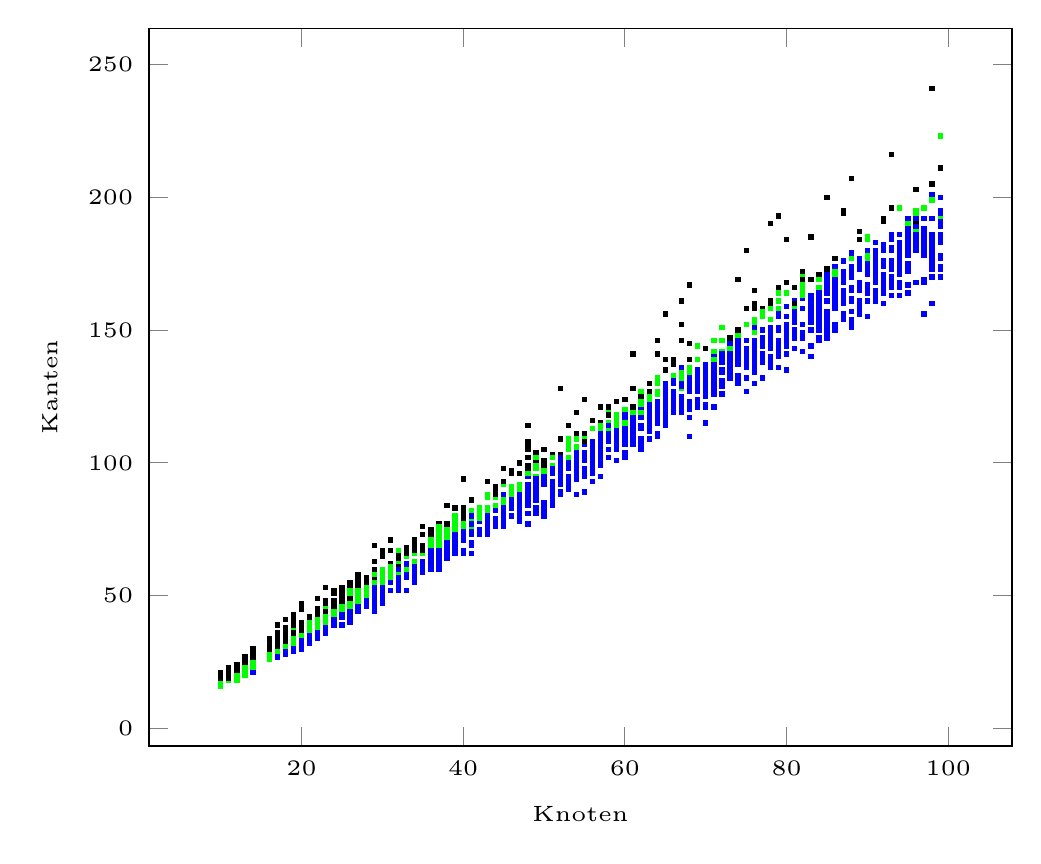
\begin{tikzpicture}[thick, scale=1.6,font=\tiny]
\begin{axis}[xlabel=Knoten,ylabel=Kanten]

\addplot[
	scatter/classes={
    	s={mark=square*,scale=0.2,black},
    	f={mark=square*,scale=0.2,green},
    	n={mark=square*,scale=0.2,blue}
    	},
	scatter,only marks,
    	scatter src=explicit symbolic,]
	table[meta=label] {
x y label
10 18 s
10 16 f
10 19 s
10 19 s
10 19 s
10 20 s
10 18 s
10 18 s
10 17 s
10 19 s
10 19 s
10 21 s
10 17 f
10 17 s
10 18 s
10 20 s
10 16 f
10 20 s
10 17 f
10 16 f
11 19 s
11 22 s
11 19 s
11 19 f
11 19 s
11 22 s
11 18 f
11 20 s
11 22 s
11 19 s
11 20 s
11 21 s
11 19 s
11 20 s
11 20 f
11 18 f
11 20 s
11 23 s
11 20 s
11 19 s
12 18 f
12 22 s
12 22 s
12 18 f
12 20 f
12 23 s
12 21 s
12 22 s
12 19 f
12 24 s
12 22 s
12 20 f
12 20 f
12 21 s
12 18 f
12 22 s
12 21 s
12 24 s
12 20 f
12 18 f
13 21 f
13 20 f
13 20 f
13 25 s
13 22 f
13 26 s
13 20 f
13 27 s
13 25 s
13 24 s
13 24 s
13 24 s
13 25 s
13 27 s
13 23 s
13 24 s
13 26 s
13 25 s
13 23 f
13 26 s
14 29 s
14 30 s
14 21 n
14 23 f
14 24 f
14 23 f
14 27 s
14 27 s
14 27 s
14 30 s
14 28 s
14 27 s
14 25 s
14 25 s
14 28 s
14 25 s
14 29 s
14 25 s
14 25 s
14 25 f
16 29 f
16 26 f
16 27 f
16 28 f
16 31 s
16 30 s
16 31 s
16 31 s
16 32 s
16 33 s
17 31 s
17 31 f
17 33 s
17 28 f
17 31 f
17 32 s
17 32 s
17 32 s
17 30 f
17 33 s
18 34 s
18 37 s
18 33 s
18 33 s
18 29 n
18 30 f
18 30 f
18 37 s
18 36 s
18 34 s
19 36 s
19 30 n
19 30 n
19 39 s
19 38 s
19 34 f
19 33 f
19 39 s
19 30 n
19 43 s
20 30 n
20 32 n
20 40 f
20 37 f
20 38 f
20 34 f
20 45 s
20 31 n
20 37 s
20 38 s
21 42 s
21 40 f
21 42 s
21 37 f
21 33 n
21 32 n
21 37 f
21 37 f
21 35 n
21 42 s
22 34 n
22 39 f
22 40 f
22 41 s
22 45 s
22 49 s
22 36 n
22 42 s
22 41 f
22 42 s
23 46 s
23 38 n
23 44 f
23 42 f
23 46 s
23 45 s
23 45 s
23 42 f
23 48 s
23 47 s
24 45 s
24 40 n
24 42 n
24 45 f
24 45 f
24 52 s
24 42 f
24 47 f
24 48 s
24 44 f
25 43 n
25 53 s
25 47 s
25 50 s
25 49 s
25 43 n
25 43 n
25 49 s
25 44 n
25 46 f
26 47 f
26 49 f
26 48 f
26 49 f
26 49 f
26 52 f
26 48 f
26 44 n
26 51 f
26 46 n
27 53 f
27 50 f
27 55 f
27 48 f
27 45 n
27 57 s
27 52 s
27 56 s
27 46 n
27 54 s
28 48 n
28 54 s
28 51 f
28 52 f
28 52 f
28 48 n
28 46 n
28 56 s
28 55 s
28 49 n
29 50 n
29 69 s
29 54 f
29 56 s
29 58 s
29 57 s
29 63 s
29 44 n
29 53 f
29 55 f
16 33 s
16 27 f
16 30 f
16 28 f
16 29 f
16 29 s
16 31 s
16 28 f
16 34 s
16 30 s
16 28 f
16 32 s
16 27 f
16 30 s
16 26 f
16 28 f
16 30 s
16 30 s
16 28 f
16 28 f
17 31 f
17 30 f
17 39 s
17 32 s
17 33 s
17 35 s
17 31 s
17 27 n
17 35 s
17 27 n
17 31 f
17 29 f
17 33 s
17 34 s
17 30 f
17 39 s
17 31 s
17 29 f
17 36 s
17 33 s
18 29 n
18 36 s
18 38 s
18 30 f
18 41 s
18 34 s
18 31 f
18 33 f
18 31 f
18 36 s
18 33 f
18 29 n
18 30 f
18 29 n
18 33 s
18 28 n
18 37 s
18 34 s
18 37 s
18 37 s
19 33 f
19 32 f
19 37 s
19 35 f
19 33 f
19 31 n
19 31 n
19 35 f
19 38 s
19 34 f
19 41 s
19 37 f
19 33 f
19 29 n
19 35 f
19 40 s
19 36 s
19 30 n
19 32 f
19 34 f
20 36 f
20 39 f
20 40 s
20 47 s
20 37 f
20 36 f
20 33 n
20 36 f
20 38 s
20 36 f
20 40 s
20 30 n
20 36 f
20 37 f
20 33 n
20 37 s
20 33 n
20 32 n
20 40 s
20 38 s
21 40 f
21 40 s
21 34 n
21 37 f
21 40 s
21 40 s
21 37 f
21 34 n
21 39 f
21 39 f
21 38 f
21 42 s
21 40 f
21 38 f
21 37 f
21 39 f
21 40 s
21 34 n
21 40 f
21 42 s
22 38 f
22 37 n
22 38 n
22 45 s
22 39 f
22 40 f
22 34 n
22 42 f
22 37 n
22 41 f
22 41 f
22 35 n
22 38 f
22 43 s
22 40 f
22 34 n
22 40 f
22 36 n
22 43 s
22 36 n
23 36 n
23 47 s
23 42 f
23 36 n
23 36 n
23 46 s
23 42 f
23 43 s
23 42 f
23 38 n
23 53 s
23 45 f
23 48 s
23 48 s
23 45 f
23 43 f
23 44 s
23 47 s
23 40 f
23 40 f
24 42 n
24 47 s
24 44 f
24 43 f
24 47 s
24 41 n
24 43 f
24 51 s
24 39 n
24 46 f
24 40 n
24 47 s
24 51 s
24 41 n
24 46 f
24 45 f
24 41 n
24 44 f
24 46 s
24 46 s
25 42 n
25 43 n
25 51 s
25 52 s
25 50 s
25 47 f
25 47 f
25 44 f
25 49 s
25 48 f
25 45 f
25 44 f
25 39 n
25 45 f
25 50 s
25 48 s
25 45 f
25 50 s
25 51 s
25 43 n
26 42 n
26 47 n
26 55 s
26 47 f
26 46 f
26 43 n
26 50 s
26 42 n
26 50 f
26 48 f
26 44 n
26 40 n
26 54 s
26 45 n
26 49 s
26 45 n
26 46 f
26 47 f
26 47 f
26 46 f
27 52 s
27 48 f
27 54 s
27 58 s
27 44 n
27 51 f
27 51 f
27 52 s
27 47 n
27 52 f
27 45 n
27 48 f
27 45 n
27 51 f
27 46 n
27 52 f
27 44 n
27 51 f
27 51 f
27 48 f
28 47 n
28 50 f
28 57 s
28 48 n
28 48 n
28 56 s
28 47 n
28 51 n
28 46 n
28 55 s
28 46 n
28 55 s
28 48 n
28 48 n
28 54 s
28 51 n
28 52 f
28 53 f
28 50 f
28 56 s
29 56 s
29 56 s
29 52 n
29 53 n
29 59 s
29 51 n
29 46 n
29 55 f
29 51 n
29 63 s
29 63 s
29 60 s
29 48 n
29 48 n
29 46 n
29 47 n
29 51 n
29 58 f
29 60 s
29 49 n
30 67 s
30 65 s
30 53 n
30 59 s
30 47 n
30 53 n
30 56 f
30 51 n
30 49 n
30 59 s
30 54 f
30 55 f
30 59 s
30 59 f
30 49 n
30 57 f
30 53 n
30 60 f
30 56 f
30 56 f
31 61 s
31 62 f
31 62 s
31 60 s
31 52 n
31 67 s
31 55 n
31 59 f
31 57 f
31 56 f
31 56 n
31 57 f
31 58 f
31 71 s
31 52 n
31 61 s
31 55 n
31 61 f
31 58 f
31 55 n
32 67 f
32 59 n
32 61 f
32 54 n
32 55 n
32 62 s
32 59 f
32 57 n
32 62 s
32 60 f
32 56 n
32 65 s
32 57 n
32 63 f
32 52 n
32 64 s
32 56 n
32 59 f
32 60 n
32 64 s
33 58 n
33 62 f
33 59 n
33 58 n
33 59 n
33 68 s
33 66 s
33 62 f
33 60 f
33 67 s
33 52 n
33 62 f
33 57 n
33 62 n
33 58 n
33 58 n
33 65 f
33 66 s
33 60 f
33 68 s
34 63 f
34 67 s
34 71 f
34 58 n
34 70 f
34 60 n
34 61 n
34 55 n
34 70 s
34 63 f
34 67 f
34 63 f
34 68 s
34 59 n
34 66 f
34 56 n
34 67 s
34 59 n
34 71 s
34 69 s
35 73 s
35 66 n
35 59 n
35 67 f
35 66 f
35 69 f
35 68 s
35 61 n
35 61 n
35 76 s
35 69 s
35 67 f
35 59 n
35 63 n
35 68 s
35 59 n
35 67 s
35 69 s
35 59 n
35 63 n
36 62 n
36 65 n
36 62 n
36 65 n
36 62 n
36 60 n
36 61 n
36 70 f
36 64 n
36 73 s
36 71 f
36 65 n
36 65 n
36 62 n
36 65 n
36 68 f
36 75 s
36 63 n
36 67 n
36 73 s
37 68 f
37 67 n
37 68 n
37 68 f
37 74 s
37 77 s
37 77 f
37 72 f
37 70 f
37 63 n
37 77 s
37 60 n
37 75 f
37 65 n
37 73 f
37 67 n
37 68 f
37 62 n
37 67 n
37 76 f
38 68 n
38 71 f
38 69 n
38 66 n
38 72 f
38 71 f
38 74 f
38 77 s
38 64 n
38 70 f
38 66 n
38 73 f
38 70 n
38 73 f
38 71 f
38 70 n
38 72 f
38 75 s
38 84 s
38 75 f
39 71 n
39 71 n
39 73 f
39 67 n
39 75 f
39 69 n
39 74 f
39 78 s
39 73 f
39 79 f
39 80 f
39 72 n
39 66 n
39 71 n
39 75 f
39 76 f
39 83 s
39 73 n
39 75 f
39 78 f
40 71 n
40 81 s
40 78 f
40 74 n
40 66 n
40 74 n
40 75 n
40 76 f
40 94 s
40 67 n
40 67 n
40 83 s
40 79 s
40 79 s
40 79 s
40 72 n
40 83 s
40 72 n
40 76 f
40 74 n
41 74 n
41 78 f
41 70 n
41 80 f
41 77 f
41 74 n
41 82 s
41 86 s
41 66 n
41 73 n
41 82 s
41 82 f
41 69 n
41 77 n
41 75 n
41 76 n
41 80 n
41 74 n
41 76 f
41 77 n
42 73 n
42 78 n
42 83 s
42 74 n
42 80 n
42 78 n
42 81 f
42 81 f
42 83 s
42 80 f
42 80 f
42 81 f
42 82 f
42 79 n
42 78 n
42 74 n
42 79 f
42 83 f
42 75 n
42 79 f
43 75 n
43 83 f
43 80 n
43 76 n
43 79 n
43 75 n
43 76 n
43 74 n
43 82 f
43 93 s
43 73 n
43 76 n
43 88 s
43 78 n
43 88 f
43 87 f
43 73 n
43 76 n
43 74 n
43 80 n
44 83 n
44 84 f
44 82 n
44 79 n
44 87 f
44 88 f
44 76 n
44 76 n
44 82 n
44 90 s
44 76 n
44 78 n
44 88 s
44 87 f
44 87 f
44 79 n
44 78 n
44 91 s
44 79 n
44 88 s
45 86 f
45 93 s
45 92 f
45 80 n
45 86 f
45 81 n
45 77 n
45 88 n
45 78 n
45 87 f
45 82 n
45 83 n
45 83 n
45 98 s
45 79 n
45 88 f
45 88 n
45 76 n
45 85 f
45 93 s
46 91 f
46 91 f
46 96 s
46 97 s
46 89 f
46 84 n
46 84 n
46 90 f
46 80 n
46 90 f
46 89 f
46 90 f
46 87 f
46 90 f
46 86 n
46 84 n
46 96 s
46 89 f
46 89 f
46 83 n
47 88 n
47 100 s
47 78 n
47 89 f
47 88 n
47 91 f
47 81 n
47 84 n
47 90 n
47 82 n
47 90 f
47 87 n
47 85 n
47 89 n
47 100 s
47 96 s
47 92 f
47 83 n
47 90 f
47 79 n
48 77 n
48 81 n
48 89 n
48 85 n
48 90 n
48 114 s
48 87 n
48 98 s
48 102 s
48 107 s
48 86 n
48 95 n
48 92 n
48 108 s
48 87 n
48 99 s
48 84 n
48 96 f
48 84 n
48 105 s
49 87 n
49 93 f
49 86 n
49 89 n
49 99 f
49 91 n
49 81 n
49 94 f
49 101 s
49 104 s
49 88 n
49 102 f
49 93 n
49 95 f
49 89 n
49 94 n
49 83 n
49 98 s
49 98 f
49 102 f
50 98 s
50 101 f
50 99 f
50 95 n
50 94 n
50 95 n
50 95 n
50 98 f
50 99 s
50 105 s
50 80 n
50 101 s
50 82 n
50 93 n
50 84 n
50 98 n
50 85 n
50 99 s
50 97 f
50 92 n
51 90 n
51 103 s
51 93 n
51 91 n
51 96 n
51 86 n
51 91 n
51 91 n
51 90 n
51 91 n
51 98 n
51 84 n
51 91 n
51 93 n
51 93 n
51 99 f
51 98 n
51 88 n
51 102 f
51 102 f
52 103 f
52 99 n
52 89 n
52 94 n
52 99 f
52 128 s
52 103 s
52 97 n
52 96 n
52 109 s
52 95 n
52 102 n
52 98 n
52 88 n
52 97 n
52 92 n
52 101 f
52 101 n
52 99 n
52 97 n
53 92 n
53 106 f
53 105 f
53 114 s
53 109 f
53 102 f
53 98 n
53 100 n
53 107 f
53 90 n
53 100 n
53 93 n
53 106 f
53 98 n
53 102 f
53 95 n
53 99 n
53 106 f
53 98 n
53 95 n
54 119 s
54 106 f
54 119 s
54 105 f
54 88 n
54 110 s
54 104 f
54 101 n
54 105 n
54 103 n
54 101 n
54 102 n
54 111 s
54 99 n
54 97 n
54 95 n
54 101 n
54 106 f
54 109 f
54 94 n
55 104 n
55 110 f
55 111 s
55 109 s
55 107 n
55 102 n
55 98 n
55 109 f
55 89 n
55 96 n
55 104 n
55 104 n
55 104 n
55 124 s
55 124 s
55 102 n
55 108 f
55 101 n
55 95 n
55 108 s
56 113 s
56 101 n
56 116 s
56 99 n
56 103 n
56 102 n
56 93 n
56 104 n
56 99 n
56 96 n
56 108 n
56 104 n
56 107 n
56 105 n
56 104 n
56 106 f
56 97 n
56 107 n
56 113 f
56 106 n
57 121 s
57 104 n
57 99 n
57 115 s
57 102 n
57 112 f
57 108 n
57 108 n
57 114 f
57 106 n
57 108 n
57 95 n
57 109 n
57 106 n
57 113 f
57 104 n
57 101 n
57 114 f
57 111 n
57 102 n
58 105 n
58 120 f
58 108 n
58 113 n
58 115 f
58 109 n
58 111 n
58 109 n
58 114 f
58 113 f
58 105 n
58 105 n
58 110 n
58 109 n
58 118 s
58 102 n
58 113 f
58 121 s
58 115 f
58 114 n
59 105 n
59 107 n
59 113 n
59 114 f
59 108 n
59 116 f
59 105 n
59 111 n
59 109 n
59 118 f
59 115 n
59 117 f
59 115 f
59 116 f
59 123 s
59 123 s
59 107 n
59 117 f
59 101 n
59 107 n
60 118 f
60 107 n
60 104 n
60 124 s
60 109 n
60 102 n
60 114 n
60 119 n
60 112 n
60 111 n
60 108 n
60 119 f
60 113 n
60 118 n
60 114 n
60 116 n
60 115 f
60 113 n
60 120 f
60 109 n
61 110 n
61 113 n
61 114 n
61 111 n
61 128 s
61 107 n
61 119 f
61 116 n
61 117 n
61 114 n
61 110 n
61 111 n
61 108 n
61 119 f
61 141 s
61 114 n
61 121 s
61 107 n
61 114 n
61 110 n
62 117 n
62 109 n
62 118 n
62 105 n
62 109 n
62 119 n
62 121 f
62 127 s
62 120 n
62 113 n
62 127 f
62 122 f
62 124 f
62 113 n
62 119 f
62 119 f
62 122 f
62 125 s
62 107 n
62 114 n
63 118 n
63 124 f
63 121 f
63 121 n
63 125 f
63 117 n
63 122 n
63 124 f
63 116 n
63 113 n
63 127 s
63 125 n
63 125 f
63 115 n
63 112 n
63 109 n
63 116 n
63 120 n
63 114 n
63 130 s
64 126 f
64 116 n
64 110 n
64 146 s
64 118 n
64 119 n
64 117 n
64 132 f
64 118 n
64 122 n
64 127 f
64 141 s
64 120 n
64 130 f
64 115 n
64 121 n
64 127 f
64 115 n
64 111 n
64 123 n
65 117 n
65 123 n
65 116 n
65 156 s
65 130 n
65 114 n
65 127 f
65 121 n
65 117 n
65 126 n
65 121 n
65 127 n
65 116 n
65 128 n
65 117 n
65 135 s
65 124 n
65 139 s
65 119 n
65 121 n
66 126 n
66 132 f
66 139 s
66 137 s
66 137 s
66 121 n
66 121 n
66 123 n
66 133 f
66 119 n
66 124 n
66 130 n
66 123 n
66 131 f
66 132 f
66 133 f
66 131 n
66 126 n
66 121 n
66 127 n
67 136 n
67 146 s
67 128 f
67 120 n
67 132 f
67 125 n
67 125 n
67 124 n
67 133 f
67 125 n
67 123 n
67 119 n
67 152 s
67 121 n
67 130 n
67 161 s
67 129 n
67 134 f
67 125 n
67 123 n
68 129 n
68 136 f
68 121 n
68 133 f
68 132 n
68 128 n
68 123 n
68 131 n
68 117 n
68 134 f
68 123 n
68 145 s
68 123 n
68 110 n
68 136 f
68 127 n
68 167 s
68 139 s
68 123 n
68 120 n
69 144 f
69 124 n
69 139 f
69 132 n
69 123 n
69 130 n
69 134 n
69 130 n
69 132 n
69 129 n
69 132 n
69 129 n
69 127 n
69 131 n
69 135 n
69 139 f
69 121 n
69 123 n
69 123 n
69 127 n
70 135 n
70 143 s
70 135 n
70 122 n
70 130 n
70 130 n
70 115 n
70 126 n
70 129 n
70 121 n
70 134 n
70 135 n
70 125 n
70 128 n
70 137 n
70 136 n
70 131 n
70 132 n
70 127 n
70 125 n
71 136 n
71 133 n
71 139 n
71 141 n
71 146 f
71 135 n
71 138 n
71 138 n
71 131 n
71 127 n
71 131 n
71 133 n
71 133 n
71 139 f
71 126 n
71 121 n
71 129 n
71 126 n
71 135 n
71 142 f
72 130 n
72 139 n
72 139 n
72 134 n
72 146 s
72 129 n
72 131 n
72 142 f
72 135 n
72 135 n
72 138 n
72 139 n
72 146 f
72 151 f
72 126 n
72 135 n
72 141 n
72 134 n
72 131 n
72 135 n
73 132 n
73 141 n
73 134 n
73 135 n
73 139 n
73 133 n
73 140 n
73 140 n
73 142 n
73 139 n
73 133 n
73 143 n
73 143 f
73 137 n
73 138 n
73 145 n
73 139 n
73 138 n
73 147 s
73 133 n
74 148 f
74 138 n
74 150 s
74 131 n
74 140 n
74 141 n
74 132 n
74 130 n
74 144 n
74 143 n
74 143 n
74 138 n
74 141 n
74 132 n
74 146 n
74 148 f
74 169 s
74 133 n
74 133 n
74 137 n
75 139 n
75 139 n
75 152 f
75 158 s
75 139 n
75 143 n
75 137 n
75 132 n
75 142 n
75 142 n
75 139 n
75 127 n
75 180 s
75 140 n
75 136 n
75 136 n
75 138 n
75 146 n
75 146 n
75 142 n
76 152 f
76 165 s
76 144 n
76 136 n
76 154 f
76 138 n
76 151 f
76 139 n
76 149 f
76 135 n
76 134 n
76 142 n
76 141 n
76 160 s
76 151 f
76 146 n
76 138 n
76 151 n
76 130 n
76 158 s
77 150 n
77 158 s
77 145 n
77 140 n
77 145 n
77 138 n
77 144 n
77 141 n
77 132 n
77 155 f
77 139 n
77 157 f
77 138 n
77 138 n
77 146 n
77 156 f
77 141 n
77 139 n
77 150 n
77 147 n
78 149 n
78 148 n
78 136 n
78 149 n
78 148 n
78 140 n
78 161 s
78 158 f
78 139 n
78 146 n
78 138 n
78 190 s
78 136 n
78 151 n
78 144 n
78 148 n
78 148 n
78 143 n
78 154 f
78 160 s
79 141 n
79 157 f
79 142 n
79 140 n
79 150 n
79 164 f
79 166 s
79 144 n
79 156 f
79 161 f
79 156 f
79 193 s
79 156 n
79 141 n
79 146 n
79 136 n
79 158 f
79 151 n
79 150 n
79 155 n
80 168 s
80 184 s
80 159 f
80 155 n
80 151 n
80 145 n
80 148 n
80 150 n
80 146 n
80 149 n
80 152 n
80 155 n
80 164 f
80 159 n
80 144 n
80 149 n
80 144 n
80 146 n
80 141 n
80 135 n
81 153 n
81 143 n
81 156 n
81 157 n
81 147 n
81 166 s
81 159 f
81 155 n
81 154 n
81 150 n
81 149 n
81 166 s
81 160 n
81 149 n
81 147 n
81 154 n
81 143 n
81 157 n
81 161 n
81 160 s
82 170 f
82 147 n
82 172 s
82 162 n
82 147 n
82 147 n
82 167 f
82 158 n
82 148 n
82 165 f
82 152 n
82 169 s
82 172 s
82 149 n
82 164 n
82 167 f
82 164 f
82 142 n
82 163 f
82 158 n
83 140 n
83 156 n
83 155 n
83 150 n
83 153 n
83 185 s
83 158 n
83 154 n
83 161 n
83 162 n
83 150 n
83 155 n
83 144 n
83 153 n
83 153 n
83 153 n
83 160 n
83 169 s
83 154 n
83 163 n
84 164 n
84 169 f
84 156 n
84 159 n
84 146 n
84 152 n
84 166 f
84 171 s
84 162 n
84 154 n
84 150 n
84 151 n
84 155 n
84 158 n
84 158 n
84 147 n
84 163 n
84 161 n
84 163 n
84 146 n
85 151 n
85 153 n
85 168 n
85 170 s
85 172 n
85 164 n
85 154 n
85 166 n
85 200 s
85 169 n
85 155 n
85 170 n
85 157 n
85 161 n
85 161 n
85 154 n
85 173 s
85 147 n
85 149 n
85 151 n
86 169 n
86 162 n
86 171 f
86 158 n
86 161 n
86 172 f
86 150 n
86 158 n
86 174 n
86 177 s
86 151 n
86 168 n
86 159 n
86 165 n
86 169 n
86 152 n
86 167 n
86 166 n
86 167 n
86 164 n
87 169 n
87 172 n
87 169 n
87 168 n
87 195 s
87 156 n
87 169 n
87 165 n
87 165 n
87 194 s
87 171 n
87 165 n
87 160 n
87 168 n
87 169 n
87 154 n
87 160 n
87 176 n
87 161 n
87 163 n
88 154 n
88 177 f
88 157 n
88 161 n
88 151 n
88 171 n
88 165 n
88 170 n
88 153 n
88 165 n
88 166 n
88 173 n
88 153 n
88 179 n
88 171 n
88 207 s
88 162 n
88 174 n
88 170 n
88 166 n
89 161 n
89 173 n
89 187 s
89 165 n
89 177 n
89 174 n
89 184 s
89 157 n
89 166 n
89 160 n
89 159 n
89 174 n
89 175 n
89 166 n
89 168 n
89 157 n
89 165 n
89 165 n
89 173 n
89 156 n
90 155 n
90 175 n
90 184 f
90 167 n
90 171 n
90 179 n
90 172 n
90 177 f
90 161 n
90 172 n
90 166 n
90 185 f
90 179 f
90 167 n
90 174 n
90 175 n
90 167 n
90 164 n
90 180 n
90 167 n
91 174 n
91 170 n
91 172 n
91 164 n
91 161 n
91 171 n
91 165 n
91 165 n
91 176 n
91 176 n
91 183 n
91 163 n
91 168 n
91 168 n
91 180 f
91 178 n
91 169 n
91 171 n
91 180 n
91 171 n
92 168 n
92 170 n
92 165 n
92 166 n
92 171 n
92 176 n
92 169 n
92 168 n
92 192 s
92 160 n
92 171 n
92 181 f
92 164 n
92 181 n
92 191 s
92 180 n
92 174 n
92 174 n
92 169 n
92 182 n
93 167 n
93 175 n
93 181 n
93 186 n
93 196 s
93 173 n
93 184 n
93 167 n
93 169 n
93 186 n
93 174 n
93 216 s
93 176 n
93 166 n
93 163 n
93 176 n
93 170 n
93 184 n
93 166 n
93 180 n
94 173 n
94 175 n
94 176 n
94 175 n
94 166 n
94 163 n
94 196 f
94 176 n
94 186 n
94 180 n
94 182 n
94 183 n
94 183 n
94 166 n
94 178 n
94 171 n
94 177 n
94 176 n
94 178 n
94 168 n
95 173 n
95 172 n
95 188 n
95 179 n
95 178 n
95 175 n
95 186 n
95 184 n
95 182 n
95 188 n
95 180 n
95 179 n
95 174 n
95 188 n
95 167 n
95 164 n
95 184 n
95 187 n
95 190 f
95 192 n
96 185 n
96 184 n
96 190 n
96 191 n
96 183 n
96 195 f
96 186 n
96 181 n
96 180 n
96 194 f
96 188 f
96 191 s
96 184 n
96 186 n
96 181 n
96 185 n
96 192 n
96 168 n
96 189 n
96 203 s
97 181 n
97 181 n
97 186 n
97 178 n
97 156 n
97 187 n
97 192 n
97 168 n
97 188 n
97 183 n
97 180 n
97 196 f
97 183 n
97 182 n
97 185 n
97 169 n
97 187 n
97 181 n
97 179 n
97 192 n
98 192 n
98 192 n
98 181 n
98 179 n
98 186 n
98 173 n
98 205 s
98 175 n
98 199 f
98 160 n
98 179 n
98 185 n
98 176 n
98 170 n
98 183 n
98 241 s
98 185 n
98 201 n
98 182 n
98 178 n
99 170 n
99 195 n
99 183 n
99 183 n
99 184 n
99 200 n
99 191 n
99 223 f
99 191 n
99 189 n
99 211 s
99 178 n
99 193 f
99 186 n
99 177 n
99 194 n
99 178 n
99 174 n
99 173 n
99 186 n
    };
\end{axis}
\end{tikzpicture}
\end{figure}

